\documentclass{standalone}
\usepackage{tikz}
\usepackage{ctex,siunitx}
\setCJKmainfont{Noto Serif CJK SC}
\usepackage{tkz-euclide}
\usepackage{amsmath}
\usetikzlibrary{patterns, calc,3d}
\usetikzlibrary {decorations.pathmorphing,decorations.pathreplacing,decorations.shapes}
\begin{document}
\small
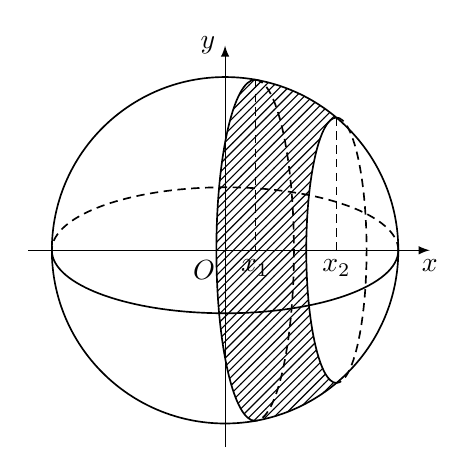
\begin{tikzpicture}[>=latex,scale=1.0]
  \draw[->](-2.5,0)--(2.6,0)node[below]{$x$};
  \draw[->](0,-2.5)--(0,2.6)node[left]{$y$};
  \draw[semithick](0,0)node[below left]{$O$}circle(2.2);
  \draw[semithick,densely dashed](2.2,0)arc(0:180:2.2 and 0.8);
  \draw[semithick](2.2,0)arc(0:-180:2.2 and 0.8);
  \draw[semithick,densely dashed]({2.2*cos(80)},{2.2*sin(80)})arc(90:-90:{0.5*sin(80)} and {2.2*sin(80)});
  \draw[semithick]({2.2*cos(80)},{2.2*sin(80)})arc(90:270:{0.5*sin(80)} and {2.2*sin(80)});
  \draw[densely dashed]({2.2*cos(80)},{2.2*sin(80)})--({2.2*cos(80)},0)node[below]{$x_1$};
  \draw[densely dashed]({2.2*cos(50)},{2.2*sin(50)})--({2.2*cos(50)},0)node[below]{$x_2$};
  \draw[semithick,densely dashed]({2.2*cos(50)},{2.2*sin(50)})arc(90:-90:{0.5*sin(50)} and {2.2*sin(50)});
  \draw[semithick]({2.2*cos(50)},{2.2*sin(50)})arc(90:270:{0.5*sin(50)} and {2.2*sin(50)});
  \fill[pattern=north east lines](50:2.2)arc(50:80:2.2)arc(90:270:{0.5*sin(80)} and {2.2*sin(80)})arc(-80:-50:2.2)arc(270:90:{0.5*sin(50)} and {2.2*sin(50)});
\end{tikzpicture}
\end{document}